\documentclass{beamer}

\usepackage{verbatim}
\usepackage{fancyvrb}
\usepackage{amsmath}
\usepackage{mathtools}
\usepackage{booktabs}
\usepackage{amssymb}
\usepackage{graphicx}
\usepackage{calc}
\usepackage{color}
\usepackage{multicol}
\usepackage{wrapfig}
\usepackage{natbib}
\usepackage[ruled,vlined]{algorithm2e}
\usepackage{animate}
\usepackage{mathtools}
\usepackage{listings}

\usepackage{cmbright}
\fontencoding{OT1}\fontfamily{cmbr}\selectfont %to load ot1cmbr.fd
\DeclareFontShape{OT1}{cmbr}{bx}{n}{% change bx definition
<->cmbrbx10%
}{}
\normalfont % back to normalfont

% two col: two columns
\newenvironment{twocol}[4]{
\begin{columns}[c]
\column{#1\textwidth}
#3
\column{#2\textwidth}
#4
\end{columns}
}

\makeatletter
\setbeamertemplate{theorem begin}
{%
\begin{\inserttheoremblockenv}
  {}{\usebeamerfont*{block title}\usebeamercolor[fg]{block title}%
  \inserttheoremname
  %\inserttheoremnumber
  \ifx \inserttheoremaddition \empty \else\ (\inserttheoremaddition)\fi
  \inserttheorempunctuation}
  \normalfont
  }
  \setbeamertemplate{theorem end}{\end{\inserttheoremblockenv}}
\makeatother

\newcommand{\E}{\mathrm{E}}
\newcommand{\Var}{\mathrm{Var}}
\newcommand{\Cov}{\mathrm{Cov}}
\newcommand{\sd}{\mathrm{sd}}
\newcommand{\s}{\mathrm{s}}
\newcommand{\Corr}{\mathrm{Corr}}
\newcommand{\rank}{\mathrm{rank}}
\newcommand{\trace}{\mathrm{trace}}
\newcommand{\nullspace}{\mathrm{null}}
\newcommand{\myspan}{\mathrm{span}}
\DeclareMathOperator*{\argmax}{arg\,max}
\DeclareMathOperator*{\argmin}{arg\,min}
\DeclareMathOperator*{\softmax}{softmax}

\definecolor{darkgreen}{rgb}{0,0.5,0}

\newtheorem{proposition}[theorem]{Proposition}
\newtheorem{exe}{Exercise}
\newtheorem{notation}{Notation}
\newtheorem{remark}{Remark}

\definecolor{darkgreen}{rgb}{0,0.5,0}

\title{Regression Models for Quantitative and Qualitative Predictors}
\author{Zhenisbek Assylbekov}
\institute{Department of Mathematics}
\date{Regression Analysis}

\AtBeginSection[]
{
  \begin{frame}<beamer>
    \tableofcontents[currentsection]
  \end{frame}
}

\begin{document}

\begin{frame}
  \titlepage
\end{frame}

\begin{frame}[fragile]{8.1 Polynomial regression}
\begin{itemize}
\item Used when the relationship between $Y$ and the predictor(s) is curvilinear.
\item\pause \structure{Example:} we might add a quadratic term to a simple linear
model to get a parabolic mean
$$
Y_i = \beta_0 + \beta_1 x_{i1} + \beta_{11} x_{i1}^2 + \epsilon_i.
$$
\item\pause We can no longer interpret $\beta_1$ and $\beta_{11}$ ``as usual.'' Cannot
hold $x_1$ constant and increase $x_1^2$ by one unit, or vice-versa!
\item\pause Can be done easily in {\sc R}, e.g. \verb|lm(y ~ x + x*x)|.
\end{itemize}
\end{frame}

\begin{frame}{General notes on fitting polynomials}
\begin{itemize}
\item Predictors can be first centered:
$$
x_{ij}^\ast = x_{ij} - \bar{x}_j,
$$ 
where $\bar{x}_j = \frac1n\sum_{i=1}^n x_{ij}$. \pause This may
reduce multicollinearity among, for example, $x_{i1}, x_{i1}^2, x_{i1}^3$, etc.
\item\pause  A polynomial $f(x) = \beta_0 + \beta_1 x + \beta_2 x^2 + \cdots + \beta_k x^k$ can have up to $k-1$ ``turning points'' or extrema. 
\item\pause A $(k-1)$th-order polynomial can go through $(x_1, Y_1), \cdots, (x_k, Y_k)$ \textit{exactly}!
\item\pause  Polynomials of degree $\ge4$  should rarely be used. \pause High-degree polynomials have
wiggly behavior and can provide extremely poor out of sample prediction. \pause Extrapolation is particularly dangerous.
\end{itemize}
\end{frame}

\begin{frame}{Polynomial regression: more than one predictor}
In the case of multiple predictors with quadratic terms,
cross-product terms should also be included, at least initially.
\vspace{10pt}

\pause \structure{Example:} Quadratic regression, two predictors:
$$
Y_i = \beta_0 + \underbrace{\beta_1 x_{i1} + \beta_2 x_{i2}}_{\text{1st order}} + \underbrace{\beta_{11} x_{i1}^2 + \beta_{22} x_{i2}^2 + \beta_{12} x_{i1} x_{i2}}_{\text{2nd order}} + \epsilon_i.
$$
\begin{itemize}
\item\pause This is an example of a \textbf{response surface}, or parabolic surface.
\item\pause ``Hierarchical model building,'' (p.~299) stipulates that a
model containing a particular term should also contain all terms of lower order including the cross-product terms.
\item\pause Degree of cross-product term is obtained by summing power 
for each predictor. E.g. the degree of $\beta_{1123} x_{i1}^2 x_{i2} x_{i3}$ is $2 + 1 + 1 = 4$.
\end{itemize}
\end{frame}

\begin{frame}{Hierarchical model building}
\begin{itemize}
\item\pause When using a polynomial regression model as an approximation to the true regression function, statisticians will
often fit a second-order or third-order model and then explore whether a lower-order model is adequate.
\item\pause With the
hierarchical approach, if a polynomial term of a given order is retained, then all related terms of lower order are also
retained in the model. 
\item\pause One would not drop the quadratic term of a predictor variable but retain the cubic
term in the model. \pause Since the quadratic term is of lower order, it is viewed as providing more basic information
about the shape of the response function; \pause the cubic term is of higher order and is viewed as providing refinements
in the specification of the shape of the response function
\end{itemize}
\end{frame}

\begin{frame}{When to include polynomial terms}
\begin{itemize}
\item If the response vs. a predictor is curved in the initial
scatterplot, this relationship \textit{may or may not hold} when other
predictors are added! \pause It's better to examine residuals versus each predictor to see if, e.g. adding a quadratic term, might be useful.
\item \pause Added variable plots are a refined plot to help figure out if the
``non-linear'' pattern is there when other variables are added (Section 10.1)
\item \pause With lots of predictors, say $k\ge5$, it is easier to reduce to
important first-order predictors, look for possible pairwise
interactions (if necessary), and then see if any of the residual
plots look curved; if so, add quadratic term(s).
\end{itemize}
\end{frame}

\begin{frame}{When to include polynomial terms}
\begin{itemize}
\item Sometimes people fit a higher-order model and then start
cutting higher order terms with $t$ and $F$-tests to get a
simpler, more interpretable model. \pause This is called \textbf{backward
elimination} (Chapter 9).
\item \pause The example on pp.~300--305 starts with a full quadratic
function:
$$
Y_i=\beta_0+\beta_1 x_1 + \beta_2 x_2 + \beta_{11}x_1^2+\beta_{12} x_1 x_2+\beta_{22}x^2+\epsilon_i
$$
\pause then throws away higher order terms through the partial F-test that FTR
$$
\text{H}_0:\,\beta_{11}=\beta_{12}=\beta_{22}=0,
$$
\pause finally leaving only the first-order terms as important:
$$
Y_i=\beta_0+\beta_1 x_1 + \beta_2 x_2 +\epsilon_i
$$
\end{itemize}
\end{frame}

\begin{frame}{8.2 Pairwise interactions among predictors}
An interaction model includes one or several \textit{cross-product} terms.\\~\\

\pause \structure{Example:} two predictors
$$
Y=\beta_0 + \beta_1 x_1 + \beta_2 x_2 + \beta_{12} x_1 x_2 + \epsilon.
$$
\pause How does the mean change when we increase $x_1$ by one unit?
\begin{align*}
\onslide<4->{\text{at $x_1$} &\Rightarrow \E[Y]=\beta_1 x_1 + \beta_2 x_2 + \beta_{12} x_1 x_2\\}
\onslide<5->{\text{at $x_1+1$} &\Rightarrow \E[Y]=\beta_1 (x_1+1) + \beta_2 x_2 + \beta_{12} (x_1+1)x_2\\}
\onslide<6->{\text{\bf difference} &= \beta_1+\beta_{12} x_2}
\end{align*}
\onslide<7->{How the mean changes depends on the other variable.}
\end{frame}

\begin{frame}{Interactions}
A model with no interactions is like a sheet of paper held ``flat.'' Adding a pairwise interaction is like twisting the two ends of the paper.
\begin{figure}
    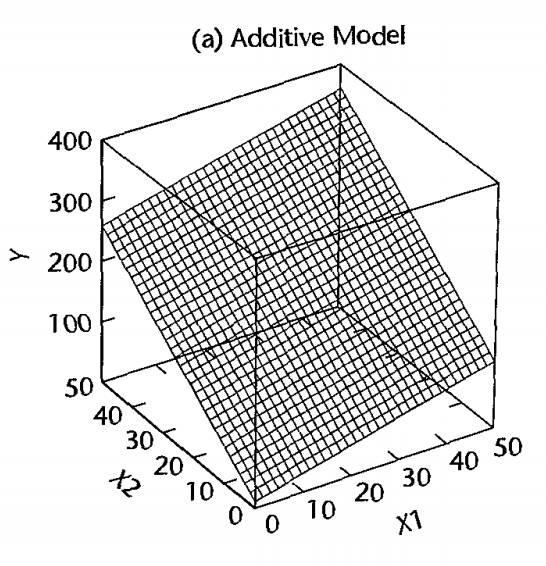
\includegraphics[height=.5\textheight]{plots/additive.png}\quad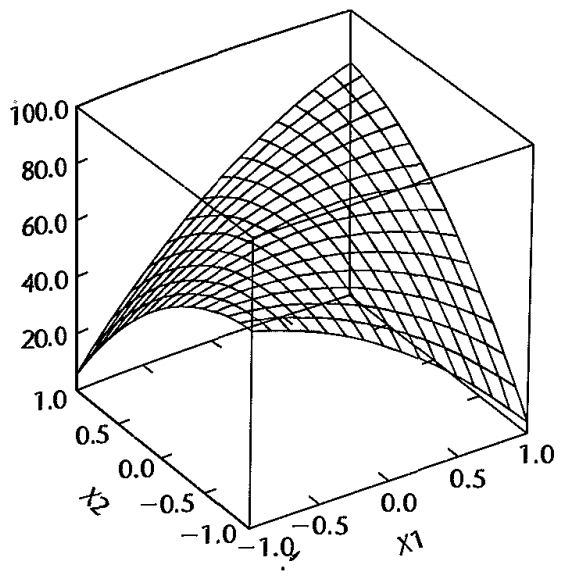
\includegraphics[height=.5\textheight]{plots/interactions.png}
    \caption{No interacations (left), With interactions (right)}
\end{figure}
\end{frame}

\begin{frame}{Interactions}
\begin{itemize}
\item Including all pairwise (or higher) interactions complicates things tremendously.
\item\pause Need to filter them out via t-tests and/or F-tests.
\item\pause The textbookook suggests fitting an additive model, then looking at residuals
$e_i$ versus each two-way interaction; \pause if there’s a pattern you
could include that the interaction should be in the model.
\item\pause A researcher will often have ``an idea''
of which variables might interact. \pause This can be helpful.
\item\pause Can also start with a first-order model, then add interactions one at a time (forward selection!) using {\sc R}.
\end{itemize}
\end{frame}

\begin{frame}[fragile]{8.3 Categorical predictors}
Let's say we wish to include a categorical variable $c$
that takes on values $c \in \{\text{category}_1, \text{category}_2, \ldots, \text{category}_l\}$. \pause We need to allow each
level of $c$ to affect $\E[Y]$ differently. \pause This is accomplished by
the use of dummy variables.\\~\\

\pause In {\sc R}, there is a way to define categorical variables; \pause then calling \verb|lm(y ~ c)| will create and handle all dummy variables automatically.\\~\\

\pause Partial F-tests can be used to see whether an entire categorical predictor can be dropped from the model (all of the dummy variables at once).
\end{frame}

\begin{frame}{Creating zero-one dummies}
Define $z_1, z_2, \ldots, z_{l-1}$ as follows:
$$
z_j=\begin{cases}
1 \quad c = \text{category}_j\\
0 \quad c \ne \text{category}_j
\end{cases}
$$
\pause This sets the last $\text{category}_l$ as the baseline. \pause Say $l=3$, then the model is
$$
\E[Y]=\beta_0+\beta_1 z_1 + \beta_2 z_2
$$
\pause which gives
\begin{align*}
&\E[Y] = \beta_0 + \beta_1&\text{when}\quad c=\text{category}_1\\
&\E[Y] = \beta_0 + \beta_2&\text{when}\quad c=\text{category}_2\\
&\E[Y] = \beta_0&\text{when}\quad c=\text{category}_3
\end{align*}
$\beta_1$ and $\beta_2$ are \textit{offsets to baseline} mean.
\end{frame}

\iffalse
\begin{frame}{Collapsing levels}
\begin{itemize}
\item Sometimes a researcher is interested in whether levels can be pooled for a categorical predictor.
\item Adding a \texttt{contrast} statement to PROC GLM will allow us to
test whether we can collapse levels. For example, for $l = 3$ we can add \texttt{contrast 'collapse 2 and 3' CAT 0 1 -1}
\end{itemize}
\end{frame}
\fi

\begin{frame}{Interaction between two categorical variables}
A two-way interaction is defined by multiplying the variables
together; \pause if one or both variables are categorical then all possible
pairings of dummy variables are considered.

\pause \structure{Example:} Say we have two categorical predictors, $x\in\{1,2,3\}$ and $z\in\{1,2,3,4\}$. An additive model is
\begin{multline*}
\E[Y]=\beta_0+\beta_1\mathbb{I}[x=1]+\beta_2\mathbb{I}[x=2] \\+\beta_3\mathbb{I}[z=1]+\beta_4\mathbb{I}[z=2]+\beta_5\mathbb{I}[z=3].
\end{multline*}
\pause The model that includes an interaction between $x$ and $z$ adds $(3-1)(4-1)=6$ additional dummy variables accounting for all possible pairwise products. \pause The new model is rather cumbersome:
\begin{footnotesize}
\begin{align*}
\E[Y]=&\beta_0+\beta_1\mathbb{I}[x=1]+\beta_2\mathbb{I}[x=2]\\
&+\beta_3\mathbb{I}[z=1]+\beta_4\mathbb{I}[z=2]+\beta_5\mathbb{I}[z=3]\\
\onslide<6->{&+\beta_6\mathbb{I}[x=1]\mathbb{I}[z=1]+\beta_7\mathbb{I}[x=1]\mathbb{I}[z=2]\\
&+\beta_8\mathbb{I}[x=1]\mathbb{I}[z=3]+\beta_9\mathbb{I}[x=2]\mathbb{I}[z=1]\\
&+\beta_{10}\mathbb{I}[x=2]\mathbb{I}[z=2]+\beta_{11}\mathbb{I}[x=2]\mathbb{I}[z=3].}
\end{align*}
\end{footnotesize}
\end{frame}


\begin{frame}[fragile]
\frametitle{Example: Insurance innovation}
An economist studied 10 mutual firms and 10 stock firms to relate speed $Y$ (months) with which an insurance innovation is adopted to size (total assets) of insurance firm $x_1$ and type $x_2$, stock or mutual.
\begin{footnotesize}
\pause \begin{verbatim}
> ins_data = read.csv("path/to/insurance.csv", header=FALSE)
> colnames(ins_data) = c('months', 'size', 'type')
> head(ins_data)
  months size   type
1     28  164  stock
2     31   85  stock
3     30  124  stock
4     21  175 mutual
5     12  210 mutual
6     15  272  stock
\end{verbatim}
\end{footnotesize}
\end{frame}


\begin{frame}{8.5 Categorical and quantitative interaction}
Consider the following model
$$
Y=\beta_0+\beta_1 x_1 +\beta_2 x_2 + \beta_{12}x_1 x_2 + \epsilon
$$
where $x_1$ is size of firm and $x_2=1$ if stock firm and $x_{2}=0$ otherwise.\\~\\

\pause Then
\begin{align*}
&\E[Y]=(\beta_0+\beta_2)+(\beta_1+\beta_{12})x_1 &\text{for stock firm}\\
&\E[Y]=\beta_0+\beta_1 x_1 &\text{otherwise}
\end{align*}
\pause Have different intercepts and different slopes. 
\end{frame}

\begin{frame}{8.5 Categorical and quantitative interaction}
If we instead fit an additive model
$$
Y=\beta_0+\beta_1 x_1 + \beta_2 x_2 + \epsilon
$$
then
\begin{align*}
&\E[Y]=(\beta_0+\beta_2)+\beta_1 x_1 &\text{for stock firm}\\
&\E[Y]=\beta_0+\beta_1 x_1 &\text{otherwise}
\end{align*}
These are two \alert{parallel} lines; the slope is the same. $\beta_2$ is how much better (or worse) stock firms do \textit{at any firm size}
\end{frame}


\begin{frame}{Insurance innovation}
\centerline{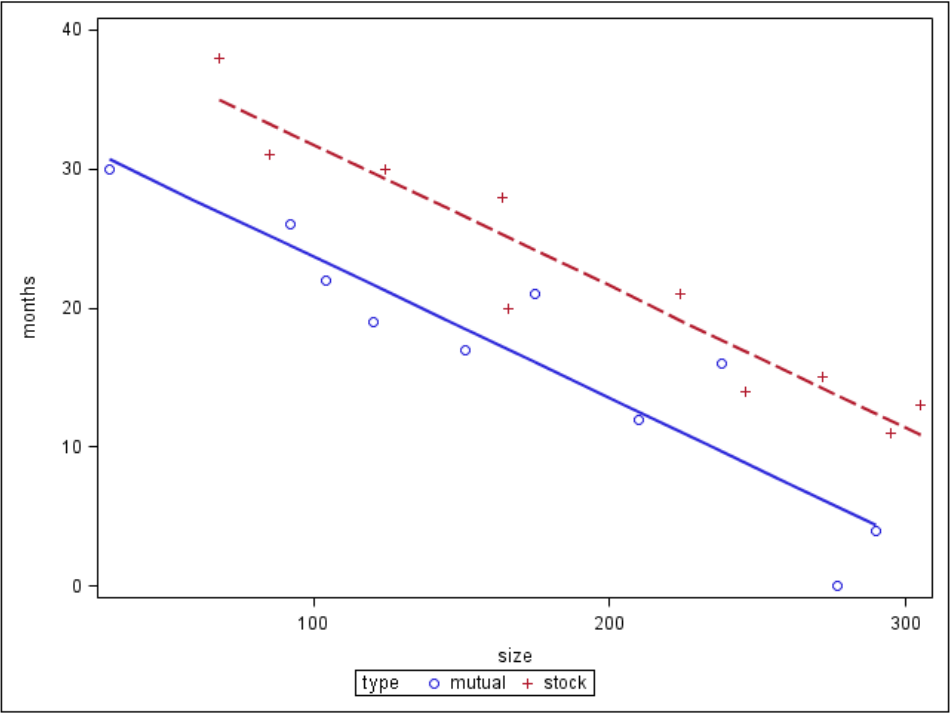
\includegraphics[scale=0.25]{categ}}
Do these look parallel?
\end{frame}

\begin{frame}[fragile]{Insurance innovation}
\begin{footnotesize}
\begin{verbatim}
> m1 = lm(months ~ size + type + size * type, data=ins_data)
> summary(m1)
...
Coefficients:
                 Estimate Std. Error t value Pr(>|t|)    
(Intercept)    33.8383695  2.4406498  13.864 2.47e-10 ***
size           -0.1015306  0.0130525  -7.779 7.97e-07 ***
typestock       8.1312501  3.6540517   2.225   0.0408 *  
size:typestock -0.0004171  0.0183312  -0.023   0.9821  

Residual standard error: 3.32 on 16 degrees of freedom
Multiple R-squared:  0.8951,	Adjusted R-squared:  0.8754 
F-statistic: 45.49 on 3 and 16 DF,  p-value: 4.675e-08 
\end{verbatim}
\end{footnotesize}
\end{frame}

\begin{frame}{Insurance innovation}
Do the following yourself:
\begin{itemize}
\item Look at standard diagnostic plots.
\item Test whether a quadratic in firm size is necessary.
\item Test whether an interaction between firm size and type is
necessary.
\item Interpret the model.
\end{itemize}
\end{frame}

\end{document}